\documentclass[11pt,addpoints]{exam}
\usepackage{enumitem}
\usepackage{amsfonts,amssymb,amsmath, amsthm}
\usepackage{graphicx}
\usepackage{systeme}
\usepackage{pgf,tikz,pgfplots}
\pgfplotsset{compat=1.15}
\usepgfplotslibrary{fillbetween}
\usepackage{mathrsfs}
\usetikzlibrary{arrows}
\usetikzlibrary{calc}
\usepackage{hyperref}
\pagestyle{headandfoot}
%\firstpageheadrule
\runningheader{Homework 2}{}{Page \thepage\ of \numpages}
\runningheadrule
\author{Aaron GK}
\usepackage{geometry}
\geometry{
	a4paper,
	total={170mm,257mm},
	left=15mm,
	right=15mm,
	bottom=20mm,
	top=15mm,
}
\firstpagefooter{}{}{}
\runningfooter{}{}{}


\begin{document}
	\title{St John Baptist De La Salle Catholic School, Addis Ababa\\
		\large Homework 5 \\
		4th Quarter}
	\maketitle
	\begin{center}
		\fbox{\fbox{\parbox{6in}{\centering
					Notes, and use of other aids is allowed.  Read all directions carefully and write your answers in the space provided.  To receive full credit, you must show all of your work. \textbf{Cheating or indications of cheating and similar answers will be punished accordingly}. 
		}}}
		\subsubsection*{Information}
		\begin{itemize}
			\item The homework is due on \textbf{Friday}, \textbf{June 16th}.
			\item You should Work on it \textbf{in groups} and consult me if you have any questions. As I have reiterated multiple times, cheating between groups will have a serious consequence.
			\item For purposes of neatness and simplicity of grading, you should do the homework on an \textbf{A-4 paper}.
		\end{itemize}
	\end{center}
	\begin{center}
		\subsection*{Questions on Electronics \& Logic Gates}
	\end{center}
	
	\begin{questions}
		\question Plot a signal for a CRO measuring a signal of frequency 250Hz and maximum voltage 10V if the gain control is 5V/cm and time base is 4ms/cm.
		\question For the logic gate shown below, show the possible outcomes for all the possible inputs.
		\begin{center}
			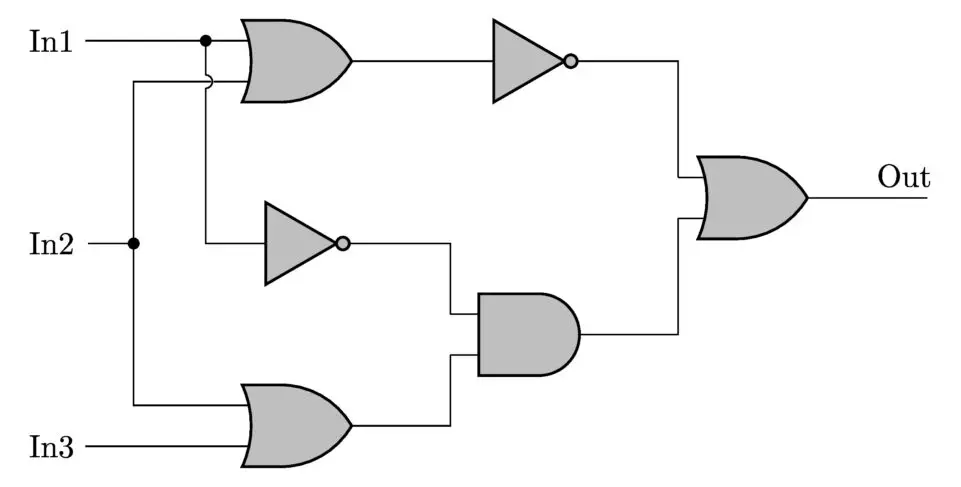
\includegraphics[scale=0.3]{lg1}
		\end{center}
		\subsection*{Advanced Problems}
		\question Explain the semiconductor band theory.
		\question How does a transistor work? Explain in detail how amplification is done.
	\end{questions}		
\end{document}